\documentclass{../template/myrpt}
\ExamName{透镜焦距的测量}
\usepackage{multirow}
\pgfplotsset{compat=1.18}

\newcolumntype{Y}{>{\centering\arraybackslash}X}
\newcolumntype{C}[1]{>{\centering\arraybackslash}m{#1}}

\begin{document}
\maketitle

\section{实验目的}
\begin{enumerate}[label=\arabic*. ]
  \item 掌握薄透镜成像的基本规律；
  \item 学习光具座上基本光路的共轴调节方法；
  \item 学会用平行光源聚焦法、物距像距法、共轭法、自准直法和成像法测量透镜焦距。
\end{enumerate}

\section{实验仪器}

主要器材包括光具座、平行白光光源（溴钨灯）、钠灯、物屏（品字屏）、像屏、凸透镜（编号 1、2、3，焦距各不相同）、凹透镜（编号 4）、平面反射镜、直尺、磁铁以及支杆、滑块和支座若干。

\section{实验原理}

\subsection{凸透镜、凹透镜的定义及常见类型}

若透镜的中心厚度远小于其球面曲率半径，可把它近似看作薄透镜。处在空气中的薄透镜按其对平行光线的作用可分为两类：一类是使平行光会聚的凸透镜，又称正透镜，其焦距取正值；另一类是使平行光发散的凹透镜，又称负透镜，其焦距取负值。

常见的凸透镜有双凸透镜、平凸透镜和正弯月透镜；常见的凹透镜有双凹透镜、平凹透镜和负弯月透镜。透镜的种类虽然不同，但在近轴条件下都可用统一的薄透镜成像规律描述其成像性质。

\subsection{薄凸透镜和薄凹透镜的成像规律}

在近轴条件下，薄透镜满足高斯成像公式
\[
  \frac{1}{u} + \frac{1}{v} = \frac{1}{f},
\]
其中 $u$ 为物距，$v$ 为像距，$f$ 为焦距。放大率为
\[
  m = -\frac{v}{u}.
\]

对凸透镜而言：当 $u > 2f$ 时成倒立缩小实像；当 $u = 2f$ 时成倒立等大实像；当 $f < u < 2f$ 时成倒立放大实像；当 $u = f$ 时出射光近似平行，不在有限距离内成像；当 $u < f$ 时成正立放大虚像。对凹透镜而言，若入射光来自实物，则通常只能形成正立、缩小的虚像。

实验中需要先调好光路共轴。共轴调节的要求是：物的中心、透镜中心和像屏中心位于同一光轴上，物面与像面垂直于光轴，导轨方向与光轴平行。只有在近轴和共轴条件较好时，薄透镜公式和各焦距测量方法才有较好的适用性。

\subsection{薄凸透镜和薄凹透镜焦距测量的方法}

\paragraph{平行光源聚焦法}
当平行光入射到凸透镜上时，出射光将在像方焦平面会聚，因此像屏上最小、最清晰的光斑对应焦点位置。此时像屏与透镜间距离就是焦距：
\[
  f = l.
\]

\paragraph{物距像距法}
在本实验的数据记录中，将同一次成像时的物距记为 $L$、像距记为 $L'$，代入高斯成像公式可得
\[
  f = \frac{LL'}{L + L'}.
\]
该方法直接、直观，但需要分别准确读取物距和像距。

\paragraph{共轭法}
固定物屏与像屏的距离 $D$，并使 $D > 4f$。此时移动凸透镜，可在光具座上找到两次清晰成像位置：一次为放大实像，一次为缩小实像。若两次清晰成像位置的间距为 $d$，则有
\[
  f = \frac{D^2 - d^2}{4D}.
\]
共轭法不必分别测量物距和像距，常用于提高凸透镜焦距测量的稳定性。

\paragraph{自准直法}
若物体位于凸透镜物方焦平面上，则透过透镜后的光成为平行光。把这束平行光经垂直于主光轴的平面镜反射回来，再次通过透镜后，会重新成像在原来的焦平面上。当返回像与物屏上的原物清晰对应时，物屏与透镜的距离即为焦距：
\[
  f = l.
\]

\paragraph{成像法测凹透镜焦距}
凹透镜不能像凸透镜那样直接把平行光会聚到实焦点上，因此实验中先用已知焦距的凸透镜形成一个实像，再把这个实像作为凹透镜的虚物。若按光传播方向取正，则凹透镜的物距 $u_2 < 0$、像距 $v_2 > 0$，仍满足
\[
  \frac{1}{u_2} + \frac{1}{v_2} = \frac{1}{f_2},
  \qquad
  f_2 = \frac{u_2 v_2}{u_2 + v_2}.
\]
测得 $u_2$ 与 $v_2$ 后即可求出凹透镜焦距 $f_2$。

\section{实验内容和步骤}

实验前先粗调和细调各光学元件的高度、左右位置与屏面方向，使物屏、透镜和像屏满足共轴要求。若成像中心不重合，可通过移动物屏中心位置和微调透镜姿态，使放大像与缩小像的中心尽量重合，再进行后续测量。

\subsection{平行光源聚焦法快速测定薄凸透镜焦距}

\begin{figure}[htbp]
  \centering
  \begin{minipage}[c]{0.42\linewidth}
    \centering
    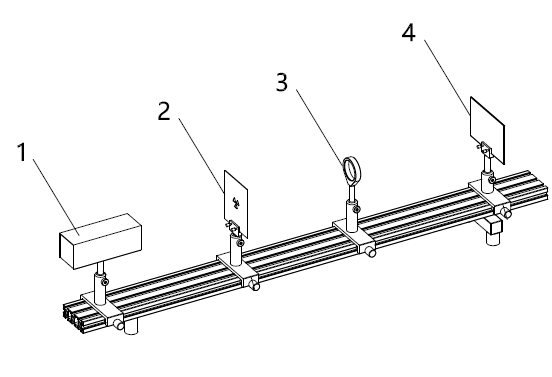
\includegraphics[width=\linewidth]{assets/parallel_setup.png}
    \par\small（a）装置示意
  \end{minipage}
  \hfill
  \begin{minipage}[c]{0.5\linewidth}
    \centering
    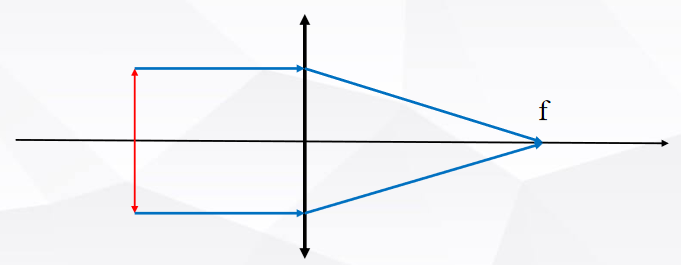
\includegraphics[width=\linewidth]{assets/parallel_ray.png}
    \par\small（b）光路示意
  \end{minipage}
  \caption{平行光源聚焦法示意}
\end{figure}

\begin{enumerate}[label=\arabic*)]
  \item 在导轨上依次放置平行白光光源、品字屏、待测凸透镜和像屏，并调至共轴。
  \item 沿导轨前后移动像屏，寻找像屏上最小、最亮且边缘最清晰的光斑位置。
  \item 记录该位置下像屏与待测凸透镜之间的距离作为焦距，重复测量两次，数据填入表 \ref{table:parallel-focus}。
\end{enumerate}

\begin{LabRecordTable}
  \centering
  \caption{平行光源聚焦法测量薄凸透镜焦距}
  \label{table:parallel-focus}
  \renewcommand{\arraystretch}{1.25}
  \setlength{\tabcolsep}{4pt}
  \small
  \begin{tabularx}{\textwidth}{C{2.2cm} Y Y Y}
    \toprule
    测量次数 & 薄凸透镜焦距 $f$/cm & 焦距平均值 $\bar{f}$/cm & 相对误差/\% \\
    \midrule
    第一次 & 7.35 & \multirow{2}{*}{7.225} & \multirow{2}{*}{3.21} \\
    第二次 & 7.10 &  &  \\
    \bottomrule
  \end{tabularx}
\end{LabRecordTable}

\subsection{物距像距法测薄凸透镜焦距}

\begin{figure}[htbp]
  \centering
  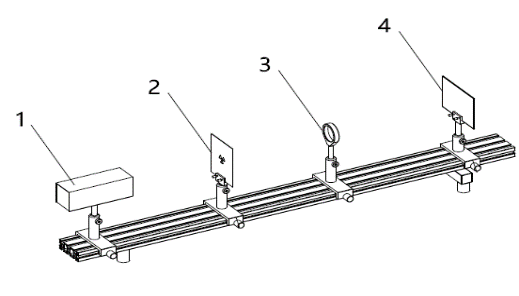
\includegraphics[width=0.58\linewidth]{assets/object_image_setup.png}
  \caption{物距像距法装置示意}
\end{figure}

\begin{enumerate}[label=\arabic*)]
  \item 在导轨上依次放置钠灯、物屏、待测凸透镜和像屏，并调至共轴。
  \item 沿导轨前后调节透镜或像屏位置，使像屏上得到清晰的实像。
  \item 读出此时的物距 $L$ 和像距 $L'$，由 $f = LL'/(L + L')$ 计算透镜焦距。
  \item 改变一次成像位置后再测量一次，将两次数据填入表 \ref{table:object-image}。
\end{enumerate}

\begin{LabRecordTable}
  \centering
  \caption{物距像距法测量薄凸透镜焦距}
  \label{table:object-image}
  \renewcommand{\arraystretch}{1.25}
  \setlength{\tabcolsep}{3.5pt}
  \small
  \begin{tabularx}{\textwidth}{C{1.9cm} *{5}{Y}}
    \toprule
    测量次数 & 物距 $L$/cm & 像距 $L'$/cm & 薄凸透镜焦距 $f$/cm & 焦距平均值 $\bar{f}$/cm & 相对误差/\% \\
    \midrule
    第一次 & 15.6 & 12.3 & 6.88 & \multirow{2}{*}{6.84} & \multirow{2}{*}{2.29} \\
    第二次 & 14.5 & 12.8 & 6.80 &  &  \\
    \bottomrule
  \end{tabularx}
\end{LabRecordTable}

\subsection{共轭法测薄凸透镜焦距}

\begin{figure}[htbp]
  \centering
  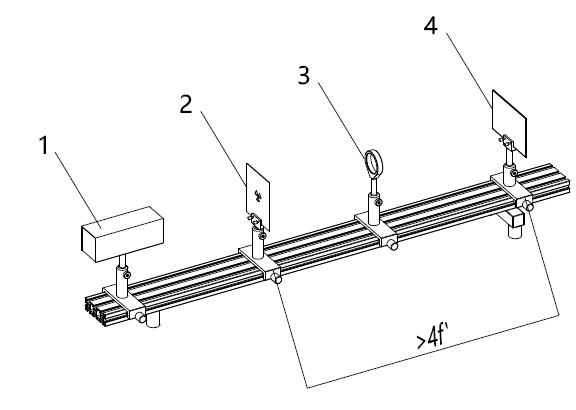
\includegraphics[width=0.62\linewidth]{assets/conjugate_setup.png}
  \caption{共轭法装置示意}
\end{figure}

\begin{enumerate}[label=\arabic*)]
  \item 在导轨上依次放置钠灯、物屏、待测凸透镜和像屏，使物屏与像屏间距 $D$ 略大于 $4f$，并保持该距离不变。
  \item 缓慢移动凸透镜位置，在像屏上先后找到放大实像和缩小实像两次清晰成像的位置，分别记为 $X_1$ 和 $X_2$。
  \item 计算两次成像位置间距 $d = |X_2 - X_1|$，再由 $f = (D^2 - d^2)/(4D)$ 求焦距。
  \item 改变一次屏间距或重新测量一次，将数据填入表 \ref{table:conjugate}。
\end{enumerate}

\begin{LabRecordTable}
  \centering
  \caption{共轭法测量薄凸透镜焦距}
  \label{table:conjugate}
  \renewcommand{\arraystretch}{1.25}
  \setlength{\tabcolsep}{2.8pt}
  \scriptsize
  \begin{tabularx}{\textwidth}{C{1.6cm} *{7}{Y}}
    \toprule
    测量次数 & 放大像位置 $X_1$/cm & 缩小像位置 $X_2$/cm & 位移 $d$/cm & 屏间距 $D$/cm & 薄凸透镜焦距 $f$/cm & 平均值 $\bar{f}$/cm & 相对误差/\% \\
    \midrule
    第一次 & 25.10 & 47.00 & 21.9 & 40.00 & 7.00 & \multirow{2}{*}{6.92} & \multirow{2}{*}{1.15} \\
    第二次 & 28.30 & 47.00 & 18.7 & 37.00 & 6.84 &  &  \\
    \bottomrule
  \end{tabularx}
\end{LabRecordTable}

\subsection{自准直法测薄凸透镜焦距}

\begin{figure}[htbp]
  \centering
  \begin{minipage}[c]{0.46\linewidth}
    \centering
    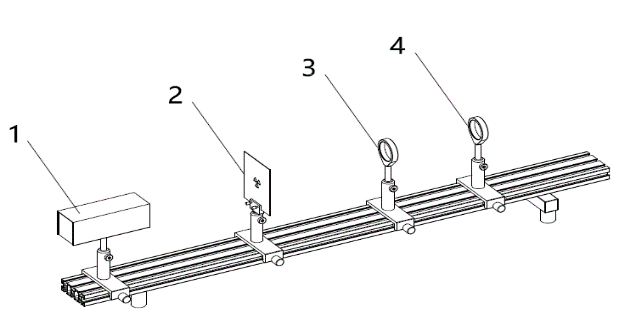
\includegraphics[width=\linewidth]{assets/autocollimation_setup.png}
    \par\small（a）装置示意
  \end{minipage}
  \hfill
  \begin{minipage}[c]{0.32\linewidth}
    \centering
    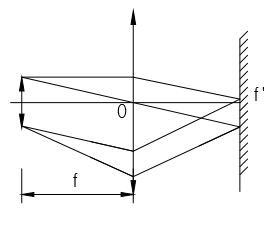
\includegraphics[width=\linewidth]{assets/autocollimation_ray.png}
    \par\small（b）光路示意
  \end{minipage}
  \caption{自准直法示意}
\end{figure}

\begin{enumerate}[label=\arabic*)]
  \item 在导轨上依次放置钠灯、物屏、待测凸透镜和平面反射镜，并调至共轴。
  \item 沿导轨前后调节物屏或待测透镜位置，使返回光在物屏上形成倒立且清晰的像。
  \item 当像最清晰、且物与像对应良好时，记录物屏与待测透镜之间的距离作为焦距。
  \item 重复测量两次，将数据填入表 \ref{table:autocollimation}。
\end{enumerate}

\begin{LabRecordTable}
  \centering
  \caption{自准直法测量薄凸透镜焦距}
  \label{table:autocollimation}
  \renewcommand{\arraystretch}{1.25}
  \setlength{\tabcolsep}{4pt}
  \small
  \begin{tabularx}{\textwidth}{C{2.2cm} Y Y Y}
    \toprule
    测量次数 & 薄凸透镜焦距 $f$/cm & 焦距平均值 $\bar{f}$/cm & 相对误差/\% \\
    \midrule
    第一次 & 6.95 & \multirow{2}{*}{6.925} & \multirow{2}{*}{1.07} \\
    第二次 & 6.90 &  &  \\
    \bottomrule
  \end{tabularx}
\end{LabRecordTable}

\subsection{成像法测凹透镜焦距}

\begin{figure}[htbp]
  \centering
  \begin{minipage}[c]{0.46\linewidth}
    \centering
    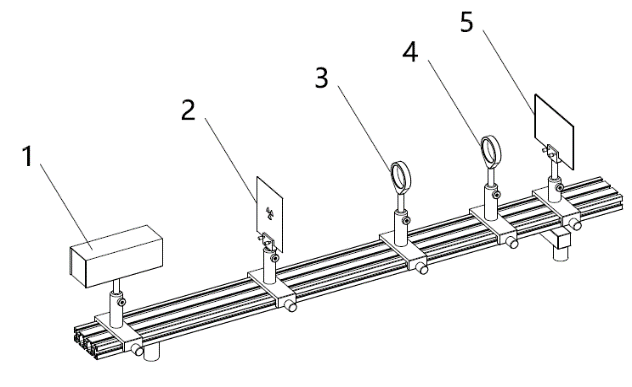
\includegraphics[width=\linewidth]{assets/concave_setup.png}
    \par\small（a）装置示意
  \end{minipage}
  \hfill
  \begin{minipage}[c]{0.4\linewidth}
    \centering
    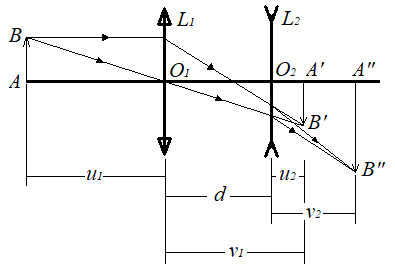
\includegraphics[width=\linewidth]{assets/concave_ray.png}
    \par\small（b）光路示意
  \end{minipage}
  \caption{成像法测量凹透镜焦距示意}
\end{figure}

\begin{enumerate}[label=\arabic*)]
  \item 按图示在导轨上依次放置钠灯、物屏、已知焦距凸透镜 $L_1$、待测凹透镜 $L_2$ 和像屏，并调至共轴。
  \item 先移开凹透镜，仅利用凸透镜 $L_1$ 使物屏在像屏上成清晰的缩小实像，记录凸透镜位置 $X_{L1}$ 和凸透镜像距 $v_1$。
  \item 保持物屏和凸透镜 $L_1$ 位置不变，在 $L_1$ 与像屏之间插入待测凹透镜 $L_2$，移动像屏重新得到清晰实像，记录凹透镜位置 $X_{L2}$ 和凹透镜像距 $v_2$。
  \item 由原来实像到凹透镜的位置求出凹透镜的物距 $u_2$，再由 $f_2 = u_2 v_2/(u_2 + v_2)$ 计算凹透镜焦距，重复测量两次并填入表 \ref{table:concave}。
\end{enumerate}

\begin{LabRecordTable}
  \centering
  \caption{成像法测量凹透镜焦距}
  \label{table:concave}
  \renewcommand{\arraystretch}{1.25}
  \setlength{\tabcolsep}{2.6pt}
  \scriptsize
  \begin{tabularx}{\textwidth}{C{1.6cm} *{8}{Y}}
    \toprule
    测量次数 & 凸透镜位置 $X_{L1}$/cm & 凸透镜像距 $v_1$/cm & 凹透镜位置 $X_{L2}$/cm & 凹透镜像距 $v_2$/cm & 凹透镜物距 $u_2$/cm & 凹透镜焦距 $f_2$/cm & 平均值 $\bar{f}_2$/cm & 相对误差/\% \\
    \midrule
    第一次 & 36.3 & 9.9 & 42.7 & 19.0 & $-3.5$ & $-4.29$ & \multirow{2}{*}{$-4.12$} & \multirow{2}{*}{17.68} \\
    第二次 & 40.0 & 9.2 & 46.0 & 17.0 & $-3.2$ & $-3.94$ &  &  \\
    \bottomrule
  \end{tabularx}
\end{LabRecordTable}

\section{实验数据处理}

本实验以待测凸透镜标称焦距 $f_0=7.00\,\mathrm{cm}$、待测凹透镜标称焦距 $f_{20}=-5.00\,\mathrm{cm}$ 作为相对误差计算的参考值。相对误差按
\[
  E_r = \frac{\left|\bar{f}-f_0\right|}{\left|f_0\right|}\times 100\%
\]
计算。

\subsection{薄凸透镜焦距}

平行光源聚焦法直接由透镜到最清晰光斑的距离得到
\[
  \bar{f}=\frac{7.35+7.10}{2}=7.225\,\mathrm{cm},
\]
相对误差为
\[
  E_r=\frac{|7.225-7.00|}{7.00}\times 100\%=3.21\%.
\]

物距像距法中，第一次测量有
\[
  f_1=\frac{LL'}{L+L'}=\frac{15.6\times 12.3}{15.6+12.3}=6.88\,\mathrm{cm},
\]
第二次测量有
\[
  f_2=\frac{14.5\times 12.8}{14.5+12.8}=6.80\,\mathrm{cm}.
\]
故平均值为 $\bar{f}=6.84\,\mathrm{cm}$，相对误差为 $2.29\%$。

共轭法中，由
\[
  f=\frac{D^2-d^2}{4D}
\]
计算得两次焦距分别为
\[
  f_1=\frac{40.00^2-21.9^2}{4\times 40.00}=7.00\,\mathrm{cm},
  \qquad
  f_2=\frac{37.00^2-18.7^2}{4\times 37.00}=6.84\,\mathrm{cm}.
\]
平均值为 $\bar{f}=6.92\,\mathrm{cm}$，相对误差为 $1.15\%$。

自准直法直接由物屏到透镜的距离得到
\[
  \bar{f}=\frac{6.95+6.90}{2}=6.925\,\mathrm{cm},
\]
相对误差为 $1.07\%$。

四种方法中，平行光源聚焦法测得的焦距最大，为 $7.225\,\mathrm{cm}$；自准直法和共轭法更接近标称值，分别为 $6.925\,\mathrm{cm}$ 和 $6.92\,\mathrm{cm}$。若取四种方法的平均值作为综合估计，则薄凸透镜焦距约为
\[
  f_{\mathrm{convex}}=\frac{7.225+6.84+6.92+6.925}{4}=6.98\,\mathrm{cm}.
\]

\subsection{薄凹透镜焦距}

成像法测凹透镜焦距时，原始记录中凹透镜物距栏记录的是原实像与凹透镜之间的几何距离。按光传播方向和薄透镜公式的符号约定，该原实像位于凹透镜入射侧的反向延长线上，作为凹透镜的虚物，因此计算时取
\[
  u_2=-3.5\,\mathrm{cm},\quad -3.2\,\mathrm{cm}.
\]
由
\[
  f_2=\frac{u_2v_2}{u_2+v_2}
\]
可得
\[
  f_{21}=\frac{(-3.5)\times 19.0}{-3.5+19.0}=-4.29\,\mathrm{cm},
  \qquad
  f_{22}=\frac{(-3.2)\times 17.0}{-3.2+17.0}=-3.94\,\mathrm{cm}.
\]
平均值为
\[
  \bar{f}_2=-4.12\,\mathrm{cm},
\]
相对误差为
\[
  E_r=\frac{|-4.12-(-5.00)|}{5.00}\times 100\%=17.68\%.
\]

\section{实验的分析和总结}

\begin{enumerate}[label=\arabic*. ]
  \item 从四种方法的结果看，物距像距法、共轭法和自准直法所得结果均在 $7.00\,\mathrm{cm}$ 附近，其中自准直法和共轭法的相对误差较小。平行光源聚焦法的结果偏大，主要原因是最小、最亮光斑位置依赖肉眼判断，光斑在焦点附近有一定亮度范围，读数容易偏向一侧。
  \item 物距像距法需要分别测量物距和像距，两个读数都会进入 $f=LL'/(L+L')$ 的计算，因此对光具座读数、透镜中心参考位置和屏面清晰程度较敏感。共轭法只需固定屏间距并测量两次成像位置间距，能部分减小物屏和像屏位置读数带来的影响，所以结果较稳定。
  \item 自准直法的优点是判据直观：返回像与原物重合且清晰时，物屏与透镜的距离即为焦距。本组数据两次测量仅相差 $0.05\,\mathrm{cm}$，重复性较好。但若平面镜未严格垂直光轴，或物屏、透镜、平面镜未调到较好的共轴状态，返回像会发生横向偏移，仍会影响焦距判断。
  \item 凹透镜焦距测量的相对误差较大。一方面，凹透镜本身不形成实焦点，需要借助凸透镜先形成实像，再把该实像作为凹透镜的虚物，光路调整和符号判断都比凸透镜测量复杂；另一方面，本组凹透镜物距绝对值只有 $3\,\mathrm{cm}$ 左右，较小的读数误差会在 $f_2=u_2v_2/(u_2+v_2)$ 中被明显放大。
\end{enumerate}

\insertSignedDataPage

\end{document}
